\documentclass[a4paper,12pt]{article}

% ===========================
% PAQUETES
% ===========================
\usepackage[utf8]{inputenc}   % Acentos
\usepackage[T1]{fontenc}
\usepackage[spanish,es-tabla,es-noshorthands]{babel}   % Idioma español ("Tabla" en vez de "Cuadro")
\usepackage{graphicx}         % Imágenes
\usepackage{fancyhdr}         % Encabezado y pie de página
\usepackage{tocloft}          % Mejor control de índices
\usepackage[table]{xcolor}    % Colores (una sola carga para evitar el "option clash")
\usepackage{booktabs}
\usepackage{float}
\usepackage[hidelinks]{hyperref}  % Después de float (si no, duplica las anclas de tablas y figuras) y antes de algorithm
\usepackage{algorithm}
\usepackage{algpseudocode}
\usepackage{multirow}
\usepackage{adjustbox}          % Tablas que no excedan el ancho de página
\usepackage{tikz}             % Diagrama de flujo de la búsqueda tabú
\usetikzlibrary{shapes.geometric,arrows.meta,positioning,calc}
\usepackage{amsmath,amssymb} % Expresiones matemáticas
\usepackage{appendix}
\usepackage[margin=2.5cm]{geometry}

\graphicspath{{imagenes/}}

% Ajuste para eliminar aviso de fancyhdr sobre headheight
\setlength{\headheight}{15pt}

% ===========================
% PSEUDOCÓDIGO EN ESPAÑOL
% ===========================
\floatname{algorithm}{Algoritmo}
\renewcommand{\listalgorithmname}{Índice de algoritmos}
\algrenewcommand\algorithmicrequire{\textbf{Entrada:}}
\algrenewcommand\algorithmicensure{\textbf{Salida:}}
\algrenewcommand\algorithmicfunction{\textbf{función}}
\algrenewcommand\algorithmicprocedure{\textbf{procedimiento}}
\algrenewcommand\algorithmicend{\textbf{fin}}
\algrenewcommand\algorithmicif{\textbf{si}}
\algrenewcommand\algorithmicthen{\textbf{entonces}}
\algrenewcommand\algorithmicelse{\textbf{si no}}
\algrenewcommand\algorithmicfor{\textbf{para}}
\algrenewcommand\algorithmicforall{\textbf{para cada}}
\algrenewcommand\algorithmicdo{\textbf{hacer}}
\algrenewcommand\algorithmicwhile{\textbf{mientras}}
\algrenewcommand\algorithmicreturn{\textbf{devolver}}
\algrenewcommand{\algorithmiccomment}[1]{\hfill $\triangleright$ \textit{#1}}

% ===========================
% ENCABEZADO Y PIE
% ===========================
\pagestyle{fancy}
\fancyhf{}
\fancyhead[L]{Práctica 1 - UJACAR (TSP)}
\fancyhead[R]{Metaheurísticas}
\fancyfoot[C]{\thepage}

\renewcommand{\appendixpagename}{Anexo}
\renewcommand{\appendixname}{Anexo}
\renewcommand{\appendixtocname}{Anexo}

\begin{document}

% ===========================
% PORTADA PERSONALIZADA
% ===========================
\hypersetup{pageanchor=false} % evita el ancla "page.1" duplicada entre la portada y el índice
\begin{titlepage}
    \centering

    % Título principal
    {\Huge \textbf{Práctica 1}\par}
    \vspace{0.3cm}
    {\Large Guion 1\par}
    \vspace{0.5cm}
    {\Large \textbf{Búsqueda Local y Trayectorias: El Viajante de Comercio (TSP)}\par}
    \vspace{1cm}
    {\Large Metaheurísticas (Curso 2026/2027)\par}
    \vspace{1cm}

    % Algoritmos implementados (exigido por la normativa de entrega)
    {\large \textbf{Algoritmos implementados:}\par}
    \vspace{0.2cm}
    Greedy $\cdot$ Greedy aleatorio $\cdot$ Búsqueda local del primer mejor (DLB) $\cdot$ Búsqueda tabú\par
    \vfill

    % Autores y universidad
    {\large \textbf{Autores:}\par}
    \vspace{0.3cm}
    \begin{tabular}{lll}
        Alejandro Ríos Cabello & arc00166 & DNI: XXXXXXXXX \\
        Nicolás Rafael Chelaru Tanase & nrct0001 & DNI: XXXXXXXXX \\
    \end{tabular}\par
    \vspace{0.5cm}
    {\large \textbf{Grupo:} XX\par}
    \vspace{1cm}

    {\large Universidad de Jaén\par}
    \vspace{0.5cm}

    % Fecha
    {\large \today\par}

    % Logo abajo
    \vfill
    \IfFileExists{imagenes/ujaen.jpg}{\includegraphics[width=0.3\textwidth]{imagenes/ujaen.jpg}}{\textbf{Universidad de Jaén}}

\end{titlepage}
\hypersetup{pageanchor=true}

\clearpage

% ===========================
% ÍNDICE GENERAL
% ===========================
\tableofcontents
\clearpage

% ===========================
% ÍNDICES DE FIGURAS Y TABLAS
% ===========================
\renewcommand{\listfigurename}{Índice de Figuras}
\renewcommand{\listtablename}{Índice de Tablas}

\listoffigures
\listoftables
\clearpage

% ===========================
% CONTENIDO (se importa de otro archivo)
% ===========================
% ===========================================================
% CONTENIDO DEL INFORME
% Las tablas de resultados (tablas/*.tex) y las figuras (imagenes/*.pdf)
% se generan con generar_resultados.py a partir de los logs.
% ===========================================================

\section{Descripción del problema}

\subsection{El problema del viajante de comercio}

El problema del viajante de comercio (TSP, \textit{Travelling Salesman Problem}) consiste en encontrar, dado un conjunto de $n$ ciudades y la distancia entre cada par de ellas, el recorrido cerrado más corto que pasa por todas las ciudades exactamente una vez y vuelve a la de origen. Se trata de un problema NP-duro. El número de recorridos distintos crece como $(n-1)!/2$, así que con las instancias que usamos (de 130 a 18.512 ciudades) no es viable una búsqueda exhaustiva y hay que recurrir a metaheurísticas.

Las instancias son de TSPLIB (\texttt{ch130}, \texttt{pr144}, \texttt{a280}, \texttt{u1060} y \texttt{d18512}). En cada fichero vienen las coordenadas $(x_i, y_i)$ de las ciudades. El problema es simétrico y la distancia entre dos ciudades es la euclídea,
\begin{equation}
d(i,j) = d(j,i) = \sqrt{(x_i - x_j)^2 + (y_i - y_j)^2}.
\end{equation}
Al leer el fichero calculamos una sola vez la matriz de distancias $D$, de tamaño $n \times n$, y así consultar una distancia durante la búsqueda cuesta $O(1)$.

\subsection{Representación de las soluciones}

Representamos cada solución como una permutación $\pi = (\pi_0, \pi_1, \dots, \pi_{n-1})$ de las ciudades $\{0, \dots, n-1\}$, donde $\pi_k$ es la ciudad que se visita en la posición $k$ del recorrido. Después de la última ciudad se vuelve a la primera, por lo que el recorrido es circular. Con esta representación cada ciudad aparece una sola vez por construcción, y todos los operadores que usamos transforman una permutación en otra.

\subsection{Función objetivo}

El objetivo es minimizar la longitud total del recorrido,
\begin{equation}
F(\pi) = \sum_{k=0}^{n-1} d\left(\pi_k, \pi_{(k+1) \bmod n}\right).
\end{equation}
Evaluar una solución completa tiene coste $O(n)$. Para medir la calidad usamos la desviación respecto al óptimo conocido de cada instancia,
\begin{equation}
\text{Desv}(\pi) = 100 \cdot \frac{F(\pi) - F^{*}}{F^{*}}.
\end{equation}

\subsection{Operadores comunes}

\paragraph{Operador de intercambio (2-opt del guion).} Dadas dos posiciones $i \neq j$, se intercambian las ciudades que hay en ellas ($\pi_i \leftrightarrow \pi_j$). Con este operador cada solución tiene $n(n-1)/2$ vecinos.

\paragraph{Evaluación factorizada.} Cuando se intercambian dos posiciones solo cambian los arcos que llegan a ellas o salen de ellas, así que el coste del vecino se puede calcular en $O(1)$ a partir del coste actual:
\begin{equation}
F(\pi') = F(\pi) - \text{arcos que desaparecen} + \text{arcos nuevos}.
\end{equation}
Si $i$ y $j$ no son adyacentes, desaparecen los cuatro arcos $(\pi_{i-1},\pi_i)$, $(\pi_i,\pi_{i+1})$, $(\pi_{j-1},\pi_j)$, $(\pi_j,\pi_{j+1})$ y aparecen otros cuatro que unen esos vecinos con la ciudad intercambiada. Si son adyacentes (por ejemplo, $j = i+1$), el arco $(\pi_i, \pi_j)$ se mantiene aunque invertido, y solo cambian los dos arcos exteriores. Los índices se toman módulo $n$. De esta forma la primera y la última posición, que en un recorrido circular también son adyacentes, se tratan igual que cualquier otro par de posiciones contiguas.

\paragraph{Don't Look Bits (DLB).} Es un vector de $n$ bits, uno por posición. Si el bit de una posición está a 0, merece la pena explorar sus intercambios, y si está a 1 es que ya se exploraron todos y ninguno mejoraba. Al principio todos valen 0. Cuando una posición agota sus movimientos sin encontrar mejora su bit pasa a 1, y vuelve a 0 si la posición participa en un movimiento que se aplica. Con esto la búsqueda se centra en las partes del recorrido que han cambiado hace poco.

\paragraph{Generación de semillas.} Partimos de la semilla base \texttt{1658743} y en cada ejecución rotamos la anterior un dígito a la izquierda, así que las tres ejecuciones usan las semillas $6587431$, $5874316$ y $8743165$. La rotación se reinicia desde la semilla base en cada algoritmo y en cada instancia, de modo que la ejecución $k$ usa la misma semilla en todos los algoritmos, tal y como pide el guion. Con la semilla se inicializa el generador \texttt{random.Random} que usan el greedy aleatorio, la búsqueda local y la búsqueda tabú, y así cualquier ejecución se puede reproducir.

\subsection{Descripción del código}

El código está hecho en Python y lo hemos dividido en estos módulos:
\begin{itemize}
    \item \texttt{main.py}: lee \texttt{parametros.txt}, carga cada instancia y lanza los algoritmos indicados en \texttt{ALGORITMO}, una vez por semilla.
    \item \texttt{extracion\_datos.py}: lee el fichero \texttt{.tsp} y calcula la matriz de distancias con NumPy.
    \item \texttt{Extraccion\_parametros.py}: lee los parámetros y genera las semillas por rotación.
    \item \texttt{Funcion\_evaluacion.py}: función objetivo, evaluación factorizada del intercambio y aplicación del movimiento.
    \item \texttt{greedy.py}, \texttt{greedy\_aleatorio.py}, \texttt{Busqueda\_local.py} y \texttt{Busqueda\_Tabu.py}: un módulo por algoritmo.
    \item \texttt{logs.py}: escribe los ficheros de registro. Los movimientos se van guardando en memoria y se escriben por bloques. El tiempo que se pierde escribiendo se resta del tiempo de ejecución que damos en los resultados.
\end{itemize}

\section{Algoritmos}

\subsection{Greedy}

Para cada ciudad calculamos la suma de sus distancias al resto, ordenamos el vector de pares $\langle$ciudad, suma$\rangle$ de menor a mayor y tomamos ese orden como recorrido. Es un algoritmo determinista y su coste es $O(n^2 + n \log n)$.

\begin{algorithm}[H]
\caption{Greedy}
\begin{algorithmic}[1]
\Require Matriz de distancias $D$ de tamaño $n$
\Ensure Recorrido $\pi$
\State $V \gets [\,]$
\For{$i \gets 0$ \textbf{hasta} $n-1$}
    \State añadir $\langle i, \sum_{j} D[i][j] \rangle$ a $V$
\EndFor
\State ordenar $V$ por la suma de forma ascendente
\State $\pi \gets$ ciudades de $V$ en ese orden
\State \Return $\pi$
\end{algorithmic}
\end{algorithm}

\subsection{Greedy aleatorio}

Usa el mismo vector ordenado, pero en cada paso escoge al azar una de las $K = 5$ primeras ciudades que quedan, la añade al recorrido y la quita del vector. Cuando quedan menos de $K$ ciudades se escoge entre las que haya.

\begin{algorithm}[H]
\caption{Greedy aleatorio}
\begin{algorithmic}[1]
\Require $D$, generador aleatorio, $K$
\Ensure Recorrido $\pi$
\State $V \gets$ vector $\langle$ciudad, suma de distancias$\rangle$ ordenado ascendentemente
\State $\pi \gets [\,]$
\While{$V$ no está vacío}
    \State $r \gets$ entero aleatorio en $[0, \min(K, |V|) - 1]$
    \State añadir la ciudad $V[r]$ a $\pi$ y eliminarla de $V$
\EndWhile
\State \Return $\pi$
\end{algorithmic}
\end{algorithm}

\subsection{Búsqueda local del primer mejor con DLB}

La búsqueda local parte de una solución del greedy aleatorio. Va recorriendo las posiciones cuyo bit DLB está a 0 y, para cada una, prueba a intercambiarla con el resto de posiciones (de forma circular, empezando en $i+1$). En cuanto encuentra un intercambio que mejora el coste lo aplica (primer mejor), reactiva los bits de las dos posiciones y vuelve a explorar la misma posición. Si no hay ninguno que mejore, desactiva su bit. El algoritmo termina cuando todos los bits están a 1, es decir, cuando se ha llegado a un óptimo local para el operador de intercambio, o cuando se alcanzan los 10.000 movimientos.

\begin{algorithm}[H]
\caption{Búsqueda local del primer mejor con DLB}
\begin{algorithmic}[1]
\Require $D$, máximo de iteraciones $M$, $K$
\Ensure Mejor recorrido encontrado
\State $\pi \gets$ GreedyAleatorio$(D, K)$; \quad $c \gets F(\pi)$
\State $dlb \gets [0, \dots, 0]$; \quad $it \gets 0$; \quad $i \gets 0$
\While{$it < M$ \textbf{y} algún $dlb[i] = 0$}
    \If{$dlb[i] = 0$}
        \State $mejora \gets$ falso
        \For{$k \gets 1$ \textbf{hasta} $n-1$}
            \State $j \gets (i + k) \bmod n$
            \If{Factorizacion$(\pi, i, j, c) < c$}
                \State intercambiar $\pi_i$ y $\pi_j$; \quad $c \gets F(\pi)$; \quad $it \gets it + 1$
                \State $dlb[i] \gets 0$; \quad $dlb[j] \gets 0$; \quad $mejora \gets$ verdadero
                \State \textbf{salir del bucle} \Comment{se vuelve a explorar la misma $i$}
            \EndIf
        \EndFor
        \If{\textbf{no} $mejora$}
            \State $dlb[i] \gets 1$; \quad $i \gets (i+1) \bmod n$
        \EndIf
    \Else
        \State $i \gets (i+1) \bmod n$
    \EndIf
\EndWhile
\State \Return $\pi$
\end{algorithmic}
\end{algorithm}

\subsection{Búsqueda tabú}

La búsqueda tabú extiende la búsqueda local para que no se pare en el primer óptimo local. Siempre se ejecutan las 10.000 iteraciones y, cuando ningún vecino permitido mejora la solución actual, se aplica el mejor vecino no tabú aunque empeore el coste (``la mejor de las peores''). Durante la búsqueda guardamos tres soluciones, que son la solución actual, el mejor del momento actual (la mejor desde el último reinicio) y el mejor global.

\paragraph{Memorias.} Para las dos memorias usamos una sola matriz $T$ de enteros de tamaño $n \times n$.
\begin{itemize}
    \item \textbf{Memoria a corto plazo (MCP)}, en el triángulo superior ($T[a][b]$ con $a < b$). Cuando se intercambian las posiciones $i$ y $j$, que contienen las ciudades $\pi_i$ y $\pi_j$, se guardan dos valores con la tenencia tabú $t = 10$. Para el par de posiciones se hace $T[\min(i,j)][\max(i,j)] \gets t$ y para el par de ciudades se hace $T[\min(\pi_i,\pi_j)][\max(\pi_i,\pi_j)] \gets t$. Un movimiento es tabú si cualquiera de sus dos celdas es mayor que 0, y en ese caso se descarta al generar el entorno. No hemos usado criterio de aspiración. Para no tener que recorrer la matriz entera en cada iteración guardamos las celdas activas en un conjunto, y en cada iteración solo se decrementan esas celdas y se quitan las que llegan a 0.
    \item \textbf{Memoria a largo plazo (MLP)}, en el triángulo inferior ($T[a][b]$ con $a > b$). En cada iteración se suma 1 a la celda de cada arco $(\pi_k, \pi_{k+1})$ de la solución actual, o sea, $n$ celdas por iteración. Al ser un problema simétrico, los arcos $(u,v)$ y $(v,u)$ comparten celda.
\end{itemize}

\paragraph{Exploración del entorno.} Se explora igual que en la búsqueda local (DLB y primer mejor), pero saltándose los movimientos tabú. Mientras se recorren los vecinos se va guardando el mejor vecino no tabú que ha aparecido. Si se encuentra una mejora se aplica, y si todos los bits del DLB acaban a 1 sin ninguna mejora se aplica ese mejor vecino. Después de aplicar un movimiento, sea del tipo que sea, solo se reactivan los bits de las dos posiciones intercambiadas. Por eso la siguiente exploración evalúa unos $2n$ vecinos y no los $n^2/2$ del entorno completo.

\paragraph{Estancamiento y oscilación estratégica.} Contamos como movimiento de empeoramiento cualquier movimiento que no mejore al mejor del momento actual. Cuando se acumulan $0{,}05 \cdot 10.000 = 500$ seguidos, consideramos que la búsqueda se ha estancado y generamos una solución nueva, por intensificación con probabilidad $0{,}5$ o por diversificación con probabilidad $0{,}5$. Los dos operadores construyen un recorrido empezando en una ciudad aleatoria. En cada paso eligen al azar entre las $K = 5$ ciudades no visitadas cuyo arco con la ciudad actual tiene mayor frecuencia en la MLP, en el caso de la intensificación, o menor frecuencia, en el de la diversificación. La intensificación reconstruye así los arcos que más han aparecido en las buenas soluciones, mientras que la diversificación lleva la búsqueda a zonas poco visitadas. Después se reinician la MCP, el DLB, el contador de estancamiento y el mejor del momento actual. La MLP se conserva.

\begin{algorithm}[H]
\caption{Búsqueda tabú}
\begin{algorithmic}[1]
\Require $D$, $M = 10.000$, $K = 5$, tenencia $t = 10$, estancamiento $e = 0{,}05$, oscilación $p = 0{,}5$
\Ensure Mejor recorrido global
\State $\pi \gets$ GreedyAleatorio$(D, K)$; \quad $\pi_{mom} \gets \pi$; \quad $\pi_{glob} \gets \pi$
\State $T \gets$ matriz $n \times n$ de ceros; \quad $dlb \gets [0, \dots, 0]$; \quad $it \gets 0$; \quad $est \gets 0$
\While{$it < M$}
    \State $(i, j) \gets$ primer movimiento no tabú que mejora $\pi$ usando el DLB
    \If{no existe}
        \State $(i, j) \gets$ mejor movimiento no tabú evaluado \Comment{la mejor de las peores}
    \EndIf
    \If{todos los movimientos evaluados son tabú}
        \State $est \gets e \cdot M$ \Comment{se fuerza el reinicio}
    \Else
        \State decrementar en 1 las celdas activas de la MCP
        \State $T[\text{posiciones } i,j] \gets t$; \quad $T[\text{ciudades } \pi_i, \pi_j] \gets t$
        \State intercambiar $\pi_i$ y $\pi_j$; \quad $dlb[i] \gets 0$; \quad $dlb[j] \gets 0$; \quad $it \gets it + 1$
        \State incrementar en la MLP los $n$ arcos de $\pi$
        \If{$F(\pi) < F(\pi_{mom})$}
            \State $\pi_{mom} \gets \pi$; \quad $est \gets 0$
            \If{$F(\pi) < F(\pi_{glob})$} $\pi_{glob} \gets \pi$ \EndIf
        \Else
            \State $est \gets est + 1$
        \EndIf
    \EndIf
    \If{$est \geq e \cdot M$}
        \If{aleatorio $< p$}
            \State $\pi \gets$ Intensificacion$(T, K)$
        \Else
            \State $\pi \gets$ Diversificacion$(T, K)$
        \EndIf
        \State $\pi_{mom} \gets \pi$; \quad actualizar $\pi_{glob}$ si $\pi$ lo mejora
        \State reiniciar MCP, $dlb$ y $est$ \Comment{la MLP no se reinicia}
    \EndIf
\EndWhile
\State \Return $\pi_{glob}$
\end{algorithmic}
\end{algorithm}

En la Figura~\ref{fig:diagrama-tabu} se muestra el mismo proceso en forma de diagrama de flujo.

% Diagrama de flujo de la búsqueda tabú (se incluye desde contenido.tex)
% "?`" es el signo de apertura de interrogación: funciona igual con pdfLaTeX y con XeTeX
\begin{figure}[H]
\centering
\begin{tikzpicture}[
    node distance=5mm and 8mm,
    every node/.style={font=\footnotesize, align=center},
    proceso/.style={rectangle, draw, rounded corners=2pt, fill=blue!6, minimum width=44mm, minimum height=7mm, inner sep=3pt},
    decision/.style={diamond, draw, fill=orange!10, aspect=2.4, inner sep=1pt},
    extremo/.style={rectangle, draw, rounded corners=8pt, fill=gray!15, minimum width=30mm, minimum height=7mm},
    flecha/.style={-{Stealth[length=2mm]}, thick},
    linea/.style={thick},
]
    % Columna principal
    \node[extremo] (inicio) {Inicio};
    \node[proceso, below=of inicio] (init) {$\pi \gets$ GreedyAleatorio$(D,K)$\\ $\pi_{mom} \gets \pi$; \ $\pi_{glob} \gets \pi$\\ $T \gets 0$; \ $dlb \gets 0$; \ $it \gets 0$; \ $est \gets 0$};
    \node[decision, below=of init] (quedan) {?`$it < M$?};
    \node[extremo, right=14mm of quedan] (fin) {Devolver $\pi_{glob}$};
    \node[proceso, below=of quedan] (explorar) {Explorar el entorno con el DLB\\ descartando los movimientos tabú};
    \node[decision, below=of explorar] (mejora) {?`Algún vecino\\ mejora $\pi$?};
    \node[proceso, below=8mm of mejora] (aplicar) {Actualizar MCP: $-1$ a los activos\\ y $t$ a posiciones y ciudades\\ Aplicar el intercambio $(i,j)$\\ $dlb[i] \gets dlb[j] \gets 0$; \ $it \gets it+1$\\ MLP: $+1$ a los $n$ arcos de $\pi$};
    \node[decision, below=of aplicar] (mommejor) {?`$F(\pi) < F(\pi_{mom})$?};
    \node[proceso, below=6mm of mommejor, xshift=-32mm, minimum width=36mm] (actmom) {$\pi_{mom} \gets \pi$; \ $est \gets 0$\\ actualizar $\pi_{glob}$ si mejora};
    \node[proceso, below=6mm of mommejor, xshift=32mm, minimum width=36mm] (incest) {$est \gets est+1$};
    \node[decision, below=24mm of mommejor] (estanca) {?`$est \geq e \cdot M$?};
    \node[decision, below=of estanca] (azar) {?`aleatorio $< p$?};
    \node[proceso, below=6mm of azar, xshift=-28mm, minimum width=36mm] (intens) {Intensificación\\ (arcos más frecuentes)};
    \node[proceso, below=6mm of azar, xshift=28mm, minimum width=36mm] (divers) {Diversificación\\ (arcos menos frecuentes)};
    \node[proceso, below=22mm of azar] (reinicio) {$\pi_{mom} \gets \pi$; \ actualizar $\pi_{glob}$ si mejora\\ Reiniciar MCP, $dlb$ y $est$ (la MLP se conserva)};

    % Rama lateral: ningún vecino mejora
    \node[decision, right=10mm of mejora] (notabu) {?`Hay vecinos\\ no tabú?};
    \node[proceso, below=8mm of notabu, minimum width=28mm] (peores) {Elegir la mejor\\ de las peores};
    \node[proceso, right=6mm of notabu, minimum width=24mm] (forzar) {$est \gets e \cdot M$\\ (forzar reinicio)};

    % Puntos de unión
    \coordinate (union1) at ($(estanca.north) + (0, 5mm)$);
    \coordinate (union2) at ($(reinicio.north) + (0, 5mm)$);
    \coordinate (bucle) at ($(actmom.west) + (-6mm, 0)$);

    % Flechas
    \draw[flecha] (inicio) -- (init);
    \draw[flecha] (init) -- (quedan);
    \draw[flecha] (quedan) -- node[right] {sí} (explorar);
    \draw[flecha] (quedan) -- node[above] {no} (fin);
    \draw[flecha] (explorar) -- (mejora);
    \draw[flecha] (mejora) -- node[right] {sí} (aplicar);
    \draw[flecha] (mejora) -- node[above] {no} (notabu);
    \draw[flecha] (notabu) -- node[right] {sí} (peores);
    \draw[flecha] (notabu) -- node[above] {no} (forzar);
    \draw[flecha] (peores) |- (aplicar);
    \draw[flecha] (aplicar) -- (mommejor);
    \draw[flecha] (mommejor.west) -| node[pos=0.3, above] {sí} (actmom.north);
    \draw[flecha] (mommejor.east) -| node[pos=0.3, above] {no} (incest.north);
    \draw[linea] (actmom.south) |- (union1);
    \draw[linea] (incest.south) |- (union1);
    \draw[linea] (forzar.south) |- (union1);
    \draw[flecha] (union1) -- (estanca.north);
    \draw[flecha] (estanca) -- node[right] {sí} (azar);
    \draw[flecha] (azar.west) -| node[pos=0.3, above] {sí} (intens.north);
    \draw[flecha] (azar.east) -| node[pos=0.3, above] {no} (divers.north);
    \draw[linea] (intens.south) |- (union2);
    \draw[linea] (divers.south) |- (union2);
    \draw[flecha] (union2) -- (reinicio.north);

    % Vueltas al inicio del bucle
    \draw[flecha] (estanca.west) -- node[above, pos=0.15] {no} (estanca.west -| bucle) |- (quedan.west);
    \draw[linea] (reinicio.west) -| (estanca.west -| bucle);
\end{tikzpicture}
\caption{Diagrama de flujo de la búsqueda tabú.}
\label{fig:diagrama-tabu}
\end{figure}


\begin{algorithm}[H]
\caption{Construcción de una solución a partir de la MLP (intensificación y diversificación)}
\begin{algorithmic}[1]
\Require MLP, $K$, modo $\in \{$intensificación, diversificación$\}$
\Ensure Recorrido $\pi$
\State $actual \gets$ ciudad aleatoria; \quad $\pi \gets [actual]$
\While{$|\pi| < n$}
    \State $f \gets$ frecuencias en la MLP de los arcos $(actual, v)$ para cada $v$ no visitada
    \If{modo = intensificación}
        \State $C \gets$ las $K$ ciudades no visitadas con mayor $f$
    \Else
        \State $C \gets$ las $K$ ciudades no visitadas con menor $f$
    \EndIf
    \State $actual \gets$ ciudad aleatoria de $C$; \quad añadir $actual$ a $\pi$
\EndWhile
\State \Return $\pi$
\end{algorithmic}
\end{algorithm}

\section{Experimentos y análisis de resultados}

\subsection{Parámetros y semillas}

Todos los parámetros se leen del fichero \texttt{parametros.txt}.

\begin{table}[H]
\centering
\begin{tabular}{lll}
\toprule
Parámetro & Valor & Algoritmos \\
\midrule
Semillas & 6587431, 5874316, 8743165 & GA, BL, Tabú \\
Ejecuciones por instancia & 3 (1 en el greedy, que es determinista) & Todos \\
$K$ & 5 & GA, BL, Tabú \\
Máximo de iteraciones & 10.000 & BL, Tabú \\
Tenencia tabú & 10 & Tabú \\
Estancamiento & 5\,\% de las iteraciones (500) & Tabú \\
Oscilación estratégica & 50\,\% & Tabú \\
\bottomrule
\end{tabular}
\caption{Parámetros de las ejecuciones.}
\label{tab:parametros}
\end{table}

En todos los algoritmos y en todas las instancias la ejecución $k$ usa la misma semilla. Así, en cada ejecución la búsqueda local y la búsqueda tabú parten de la misma solución del greedy aleatorio y sus resultados se pueden comparar directamente. Los tiempos se han medido todos en el mismo equipo y no incluyen la escritura de los logs.

\subsection{Resultados}

En las Tablas~\ref{tab:gre-res} a~\ref{tab:tabu-res} aparecen el coste y el tiempo de cada ejecución, además del mejor y el peor valor, la media y la desviación típica. La Tabla~\ref{tab:resumen} resume la desviación media respecto al óptimo y el tiempo medio. Como óptimos hemos tomado ch130 = 6.110, pr144 = 58.537, a280 = 2.579, u1060 = 224.094 y d18512 = 645.238.

% Generado por generar_resultados.py a partir de logs/: no editar a mano
\begin{table}[H]
\centering\small\setlength{\tabcolsep}{4pt}\renewcommand{\arraystretch}{1.15}
\begin{adjustbox}{max width=\textwidth}
\begin{tabular}{lrrr}
\toprule
Instancia & Coste & Desv. (\%) & Tiempo (s) \\
\midrule
\rowcolor{gray!10}ch130 & 40{.}397{,}47 & 561{,}17 & $<$\,0{,}001 \\
pr144 & 640{.}770{,}87 & 994{,}64 & $<$\,0{,}001 \\
\rowcolor{gray!10}a280 & 30{.}296{,}82 & 1{.}074{,}75 & 0{,}001 \\
u1060 & 5{.}670{.}064{,}52 & 2{.}430{,}22 & 0{,}003 \\
\rowcolor{gray!10}d18512 & 51{.}161{.}687{,}44 & 7{.}829{,}12 & 0{,}171 \\
\bottomrule
\end{tabular}
\end{adjustbox}
\caption[Resultados de Greedy]{Resultados de Greedy (determinista: una sola ejecución por instancia).}
\label{tab:gre-res}
\end{table}

% Generado por generar_resultados.py a partir de logs/: no editar a mano
\begin{table}[H]
\centering\small\setlength{\tabcolsep}{4pt}\renewcommand{\arraystretch}{1.15}
\begin{adjustbox}{max width=\textwidth}
\begin{tabular}{llrrrrrrr}
\toprule
 & & \multicolumn{3}{c}{Ejecución} & \multicolumn{4}{c}{Estadísticos} \\
\cmidrule(lr){3-5}\cmidrule(lr){6-9}
Instancia & & 1 & 2 & 3 & Mejor & Peor & Media & Desv. típ. \\
\midrule
\rowcolor{gray!10}ch130 & Coste & 41{.}107 & 41{.}379 & 40{.}198 & 40{.}198 & 41{.}379 & 40{.}894 & 618 \\
\rowcolor{gray!10} & Tiempo (s) & 0{,}001 & 0{,}001 & 0{,}001 & 0{,}001 & 0{,}001 & 0{,}001 & $<$\,0{,}001 \\
pr144 & Coste & 644{.}001 & 748{.}053 & 688{.}917 & 644{.}001 & 748{.}053 & 693{.}657 & 52{.}188 \\
 & Tiempo (s) & 0{,}001 & 0{,}001 & 0{,}001 & 0{,}001 & 0{,}001 & 0{,}001 & $<$\,0{,}001 \\
\rowcolor{gray!10}a280 & Coste & 29{.}923 & 29{.}455 & 30{.}283 & 29{.}455 & 30{.}283 & 29{.}887 & 415 \\
\rowcolor{gray!10} & Tiempo (s) & 0{,}002 & 0{,}002 & 0{,}002 & 0{,}002 & 0{,}002 & 0{,}002 & $<$\,0{,}001 \\
u1060 & Coste & 5{.}432{.}361 & 5{.}726{.}073 & 5{.}611{.}772 & 5{.}432{.}361 & 5{.}726{.}073 & 5{.}590{.}068 & 148{.}054 \\
 & Tiempo (s) & 0{,}020 & 0{,}020 & 0{,}020 & 0{,}020 & 0{,}020 & 0{,}020 & $<$\,0{,}001 \\
\rowcolor{gray!10}d18512 & Coste & 51{.}931{.}042 & 51{.}597{.}814 & 50{.}934{.}175 & 50{.}934{.}175 & 51{.}931{.}042 & 51{.}487{.}677 & 507{.}478 \\
\rowcolor{gray!10} & Tiempo (s) & 7{,}354 & 8{,}061 & 7{,}389 & 7{,}354 & 8{,}061 & 7{,}601 & 0{,}398 \\
\bottomrule
\end{tabular}
\end{adjustbox}
\caption[Resultados de Greedy aleatorio]{Resultados de Greedy aleatorio: coste y tiempo de cada ejecución (semillas 6587431, 5874316, 8743165, iguales en todas las instancias). Mejor y peor: menor y mayor valor de la fila. Costes redondeados a la unidad.}
\label{tab:grea-res}
\end{table}

% Generado por generar_resultados.py a partir de logs/: no editar a mano
\begin{table}[H]
\centering\scriptsize\setlength{\tabcolsep}{3pt}
\resizebox{\textwidth}{!}{%
\begin{tabular}{lrrrrrrrrrr}
\toprule
 & \multicolumn{2}{c}{ch130} & \multicolumn{2}{c}{pr144} & \multicolumn{2}{c}{a280} & \multicolumn{2}{c}{u1060} & \multicolumn{2}{c}{d18512} \\
 & Coste & T (s) & Coste & T (s) & Coste & T (s) & Coste & T (s) & Coste & T (s) \\
\midrule
Ejecución 1 & 13{.}868{,}04 & 0{,}091 & 222{.}961{,}32 & 0{,}104 & 6{.}092{,}60 & 0{,}567 & 679{.}598{,}50 & 11{,}552 & 50{.}148{.}233{,}54 & 78{,}626 \\
Ejecución 2 & 12{.}709{,}21 & 0{,}097 & 204{.}411{,}47 & 0{,}104 & 7{.}488{,}31 & 0{,}583 & 812{.}103{,}44 & 12{,}184 & 51{.}170{.}029{,}17 & 78{,}715 \\
Ejecución 3 & 12{.}099{,}93 & 0{,}101 & 222{.}428{,}84 & 0{,}117 & 6{.}848{,}08 & 0{,}548 & 780{.}085{,}34 & 12{,}598 & 50{.}828{.}025{,}85 & 78{,}905 \\
\midrule
Media & 12{.}892{,}39 & 0{,}096 & 216{.}600{,}54 & 0{,}108 & 6{.}809{,}66 & 0{,}566 & 757{.}262{,}43 & 12{,}111 & 50{.}715{.}429{,}52 & 78{,}749 \\
Desv. típica & 898{,}17 & 0{,}005 & 10{.}559{,}40 & 0{,}008 & 698{,}65 & 0{,}018 & 69{.}137{,}93 & 0{,}527 & 520{.}120{,}20 & 0{,}143 \\
\bottomrule
\end{tabular}}
\caption{Resultados de Búsqueda local (semillas por instancia, en orden de ejecución: ch130: 8743165/7431658/4316587, pr144: 7431658/4316587/3165874, a280: 6587431/5874316/8743165, u1060: 3165874/1658743/6587431, d18512: 1658743/6587431/5874316).}
\label{tab:b_local-res}
\end{table}

% Generado por generar_resultados.py a partir de logs/: no editar a mano
\begin{table}[H]
\centering\scriptsize\setlength{\tabcolsep}{3pt}
\resizebox{\textwidth}{!}{%
\begin{tabular}{lrrrrrrrrrr}
\toprule
 & \multicolumn{2}{c}{ch130} & \multicolumn{2}{c}{pr144} & \multicolumn{2}{c}{a280} & \multicolumn{2}{c}{u1060} & \multicolumn{2}{c}{d18512} \\
 & Coste & T (s) & Coste & T (s) & Coste & T (s) & Coste & T (s) & Coste & T (s) \\
\midrule
Ejecución 1 & 9{.}010{,}83 & 4{,}797 & 127{.}137{,}85 & 5{,}144 & 4{.}794{,}62 & 10{,}855 & 771{.}797{,}69 & 16{,}780 & 50{.}888{.}200{,}00 & 112{,}955 \\
Ejecución 2 & 7{.}791{,}07 & 5{,}245 & 102{.}932{,}41 & 6{,}204 & 4{.}873{,}41 & 10{,}737 & 732{.}013{,}31 & 16{,}351 & 50{.}671{.}520{,}00 & 102{,}665 \\
Ejecución 3 & 8{.}332{,}04 & 4{,}466 & 113{.}961{,}23 & 4{,}773 & 4{.}866{,}40 & 10{,}528 & 745{.}916{,}94 & 21{,}065 & 50{.}122{.}332{,}00 & 105{,}228 \\
\midrule
Media & 8{.}377{,}98 & 4{,}836 & 114{.}677{,}16 & 5{,}374 & 4{.}844{,}81 & 10{,}707 & 749{.}909{,}31 & 18{,}065 & 50{.}560{.}684{,}00 & 106{,}949 \\
Desv. típica & 611{,}18 & 0{,}391 & 12{.}118{,}59 & 0{,}742 & 43{,}60 & 0{,}165 & 20{.}190{,}43 & 2{,}606 & 394{.}780{,}84 & 5{,}357 \\
\bottomrule
\end{tabular}}
\caption{Resultados de Búsqueda tabú (semillas por instancia, en orden de ejecución: ch130: 1658743/6587431/5874316, pr144: 7431658/4316587/3165874, a280: 6587431/5874316/8743165, u1060: 8743165/7431658/4316587, d18512: 6587431/5874316/8743165).}
\label{tab:tabu-res}
\end{table}

% Generado por generar_resultados.py a partir de logs/: no editar a mano
\begin{table}[H]
\centering\scriptsize\setlength{\tabcolsep}{3pt}
\resizebox{\textwidth}{!}{%
\begin{tabular}{lrrrrrrrrrrrr}
\toprule
 & \multicolumn{2}{c}{ch130} & \multicolumn{2}{c}{pr144} & \multicolumn{2}{c}{a280} & \multicolumn{2}{c}{u1060} & \multicolumn{2}{c}{d18512} & \multicolumn{2}{c}{Media} \\
 & Desv (\%) & T (s) & Desv (\%) & T (s) & Desv (\%) & T (s) & Desv (\%) & T (s) & Desv (\%) & T (s) & Desv (\%) & T (s) \\
\midrule
Greedy & 561{,}17 & 0{,}000 & 994{,}64 & 0{,}000 & 1{.}074{,}75 & 0{,}001 & 2{.}430{,}22 & 0{,}002 & 7{.}829{,}12 & 0{,}160 & 2{.}577{,}98 & 0{,}033 \\
Greedy aleatorio & 582{,}70 & 0{,}001 & 1{.}030{,}13 & 0{,}001 & 1{.}062{,}92 & 0{,}002 & 2{.}375{,}73 & 0{,}024 & 7{.}879{,}64 & 8{,}724 & 2{.}586{,}22 & 1{,}750 \\
Búsqueda local & 111{,}00 & 0{,}096 & 270{,}02 & 0{,}108 & 164{,}04 & 0{,}566 & 237{,}92 & 12{,}111 & 7{.}759{,}96 & 78{,}749 & 1{.}708{,}59 & 18{,}326 \\
Búsqueda tabú & 45{,}97 & 4{,}508 & 100{,}89 & 4{,}789 & 72{,}23 & 9{,}187 & 256{,}81 & 14{,}871 & 7{.}729{,}20 & 77{,}037 & 1{.}641{,}02 & 22{,}079 \\
\bottomrule
\end{tabular}}
\caption{Desviación media respecto al óptimo y tiempo medio por algoritmo e instancia.}
\label{tab:resumen}
\end{table}


\begin{figure}[H]
\centering
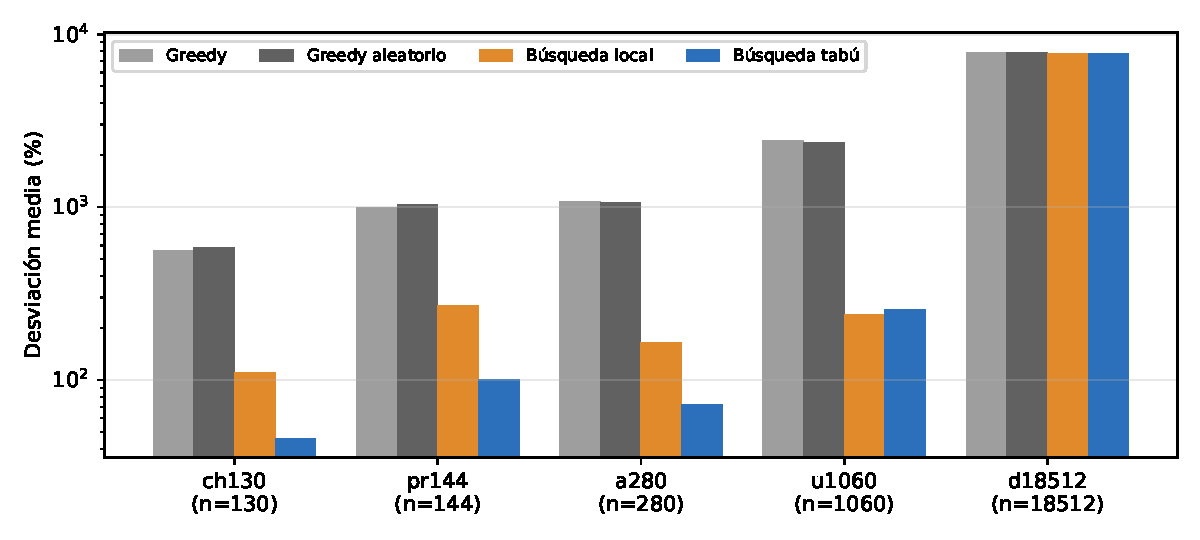
\includegraphics[width=\textwidth]{desviacion.pdf}
\caption{Desviación media respecto al óptimo por algoritmo e instancia (escala logarítmica).}
\label{fig:desviacion}
\end{figure}

\begin{figure}[H]
\centering
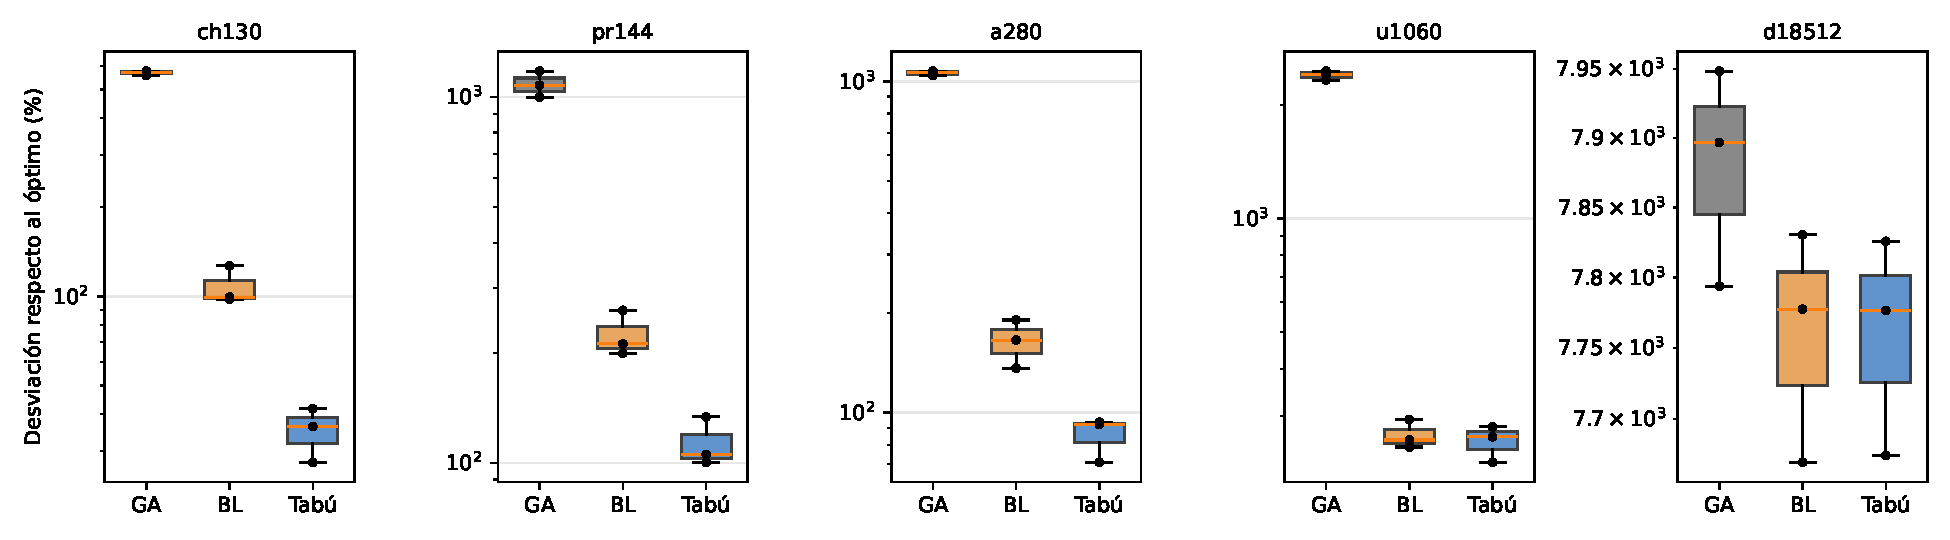
\includegraphics[width=\textwidth]{boxplot.pdf}
\caption{Distribución de la desviación de las ejecuciones del greedy aleatorio (GA), la búsqueda local (BL) y la búsqueda tabú. Cada punto es una ejecución.}
\label{fig:boxplot}
\end{figure}

\subsection{Análisis de los algoritmos}

\paragraph{Greedy y greedy aleatorio.} Los dos dan recorridos entre 6 y 80 veces más largos que el óptimo (Tabla~\ref{tab:resumen}). El problema está en el criterio de construcción. Al ordenar las ciudades por la suma de sus distancias al resto quedan primero las ciudades centrales y después las periféricas, pero en ningún momento se mira si dos ciudades consecutivas del recorrido están cerca. Por eso el recorrido va saltando de un extremo a otro del plano. Que el greedy aleatorio elija al azar entre las $K = 5$ siguientes no arregla esto. Su media queda muy cerca de la del greedy (entre un 1\,\% mejor y un 8\,\% peor según la instancia) y lo único que añade es dispersión (Figura~\ref{fig:boxplot}). Lo que tiene de útil es que es instantáneo y que da soluciones iniciales distintas para las búsquedas basadas en trayectorias.

\paragraph{Búsqueda local.} En las cuatro instancias menores reduce la desviación del greedy aleatorio entre 4,8 y 9 veces. En la Tabla~\ref{tab:bl-parada} se ve por qué es tan rápida en las pequeñas. En ch130, pr144 y a280 llega a un óptimo local después de unos 500--1.600 movimientos y para en menos de un segundo, ya que ningún intercambio mejora la solución. Ese óptimo local sigue estando lejos del global (98--261\,\% de desviación) porque el operador de intercambio es poco potente para el TSP. Al mover dos ciudades cambian cuatro arcos a la vez y casi nunca se deshace un cruce entre aristas, que es el defecto típico de un recorrido malo (Figura~\ref{fig:recorridos}).

% Generado por generar_resultados.py a partir de logs/: no editar a mano
\begin{table}[H]
\centering\small
\begin{tabular}{lrrl}
\toprule
Instancia & Ejec. & Movimientos & Motivo de parada \\
\midrule
ch130 & 1 & 493 & no se encontraron más movimientos de mejora \\
ch130 & 2 & 541 & no se encontraron más movimientos de mejora \\
ch130 & 3 & 560 & no se encontraron más movimientos de mejora \\
pr144 & 1 & 515 & no se encontraron más movimientos de mejora \\
pr144 & 2 & 554 & no se encontraron más movimientos de mejora \\
pr144 & 3 & 593 & no se encontraron más movimientos de mejora \\
a280 & 1 & 1{.}634 & no se encontraron más movimientos de mejora \\
a280 & 2 & 1{.}550 & no se encontraron más movimientos de mejora \\
a280 & 3 & 1{.}509 & no se encontraron más movimientos de mejora \\
u1060 & 1 & 9{.}383 & no se encontraron más movimientos de mejora \\
u1060 & 2 & 9{.}340 & no se encontraron más movimientos de mejora \\
u1060 & 3 & 9{.}866 & no se encontraron más movimientos de mejora \\
d18512 & 1 & 10{.}000 & alcanzado el máximo de movimientos \\
d18512 & 2 & 10{.}000 & alcanzado el máximo de movimientos \\
d18512 & 3 & 10{.}000 & alcanzado el máximo de movimientos \\
\bottomrule
\end{tabular}
\caption{Movimientos realizados por la búsqueda local y motivo de parada.}
\label{tab:bl-parada}
\end{table}


\paragraph{Búsqueda tabú.} Es el mejor algoritmo en ch130, pr144 y a280, con una desviación media entre 1,9 y 3,1 veces menor que la de la búsqueda local. El motivo se ve en la Tabla~\ref{tab:tabu}, porque en estas instancias más o menos un tercio de las 10.000 iteraciones son movimientos de empeoramiento. Como acepta ``la mejor de las peores'' y prohíbe deshacer el movimiento durante 10 iteraciones, la búsqueda consigue salir del óptimo local en el que se habría quedado la búsqueda local y sigue bajando por otra zona. En 6 de las 9 ejecuciones la mejor solución global aparece después de la iteración 7.000, mucho después de que la búsqueda local hubiera terminado.

En la Figura~\ref{fig:convergencia} se ve bien este comportamiento. En ch130 las dos ejecuciones que aparecen usan la misma semilla y parten de la misma solución, así que sus curvas coinciden mientras las dos bajan. La búsqueda local se para hacia la iteración 550 y el tabú sigue mejorando poco a poco. Los picos de la solución actual son los reinicios por estancamiento (Tabla~\ref{tab:tabu}). Las soluciones que salen de la diversificación empiezan muy lejos del mejor coste, porque construyen el recorrido con los arcos menos usados, y a partir de ellas la búsqueda vuelve a bajar. Los reinicios por intensificación empiezan en costes mucho más bajos al reutilizar los arcos que más se han repetido. En ch130 sus soluciones iniciales cuestan entre 20.550 y 22.480, mientras que las de diversificación cuestan 50.520--55.200.

% Generado por generar_resultados.py a partir de logs/: no editar a mano
\begin{table}[H]
\centering\small
\begin{tabular}{lrrrrr}
\toprule
Instancia & Ejec. & Empeoramientos & Reinicios (I/D) & Última mejora global & Coste final \\
\midrule
ch130 & 1 & 3{.}556 & 4 (2/2) & 9{.}047 & 9{.}010{,}83 \\
ch130 & 2 & 3{.}607 & 3 (1/2) & 7{.}354 & 7{.}791{,}07 \\
ch130 & 3 & 3{.}301 & 4 (1/3) & 8{.}765 & 8{.}332{,}04 \\
pr144 & 1 & 3{.}403 & 5 (3/2) & 4{.}226 & 127{.}137{,}85 \\
pr144 & 2 & 3{.}818 & 3 (2/1) & 7{.}879 & 102{.}932{,}41 \\
pr144 & 3 & 3{.}192 & 5 (2/3) & 4{.}259 & 113{.}961{,}23 \\
a280 & 1 & 3{.}417 & 1 (1/0) & 9{.}715 & 4{.}794{,}62 \\
a280 & 2 & 3{.}501 & 1 (1/0) & 7{.}331 & 4{.}873{,}41 \\
a280 & 3 & 3{.}542 & 2 (1/1) & 9{.}339 & 4{.}866{,}40 \\
u1060 & 1 & 24 & 0 (0/0) & 10{.}000 & 771{.}797{,}69 \\
u1060 & 2 & 18 & 0 (0/0) & 9{.}998 & 732{.}013{,}31 \\
u1060 & 3 & 376 & 0 (0/0) & 9{.}862 & 745{.}916{,}94 \\
d18512 & 1 & 496 & 0 (0/0) & 9{.}999 & 50{.}888{.}200{,}00 \\
d18512 & 2 & 510 & 0 (0/0) & 10{.}000 & 50{.}671{.}520{,}00 \\
d18512 & 3 & 532 & 0 (0/0) & 10{.}000 & 50{.}122{.}332{,}00 \\
\bottomrule
\end{tabular}
\caption{Comportamiento interno de la búsqueda tabú (10.000 iteraciones por ejecución).}
\label{tab:tabu}
\end{table}


\begin{figure}[H]
\centering
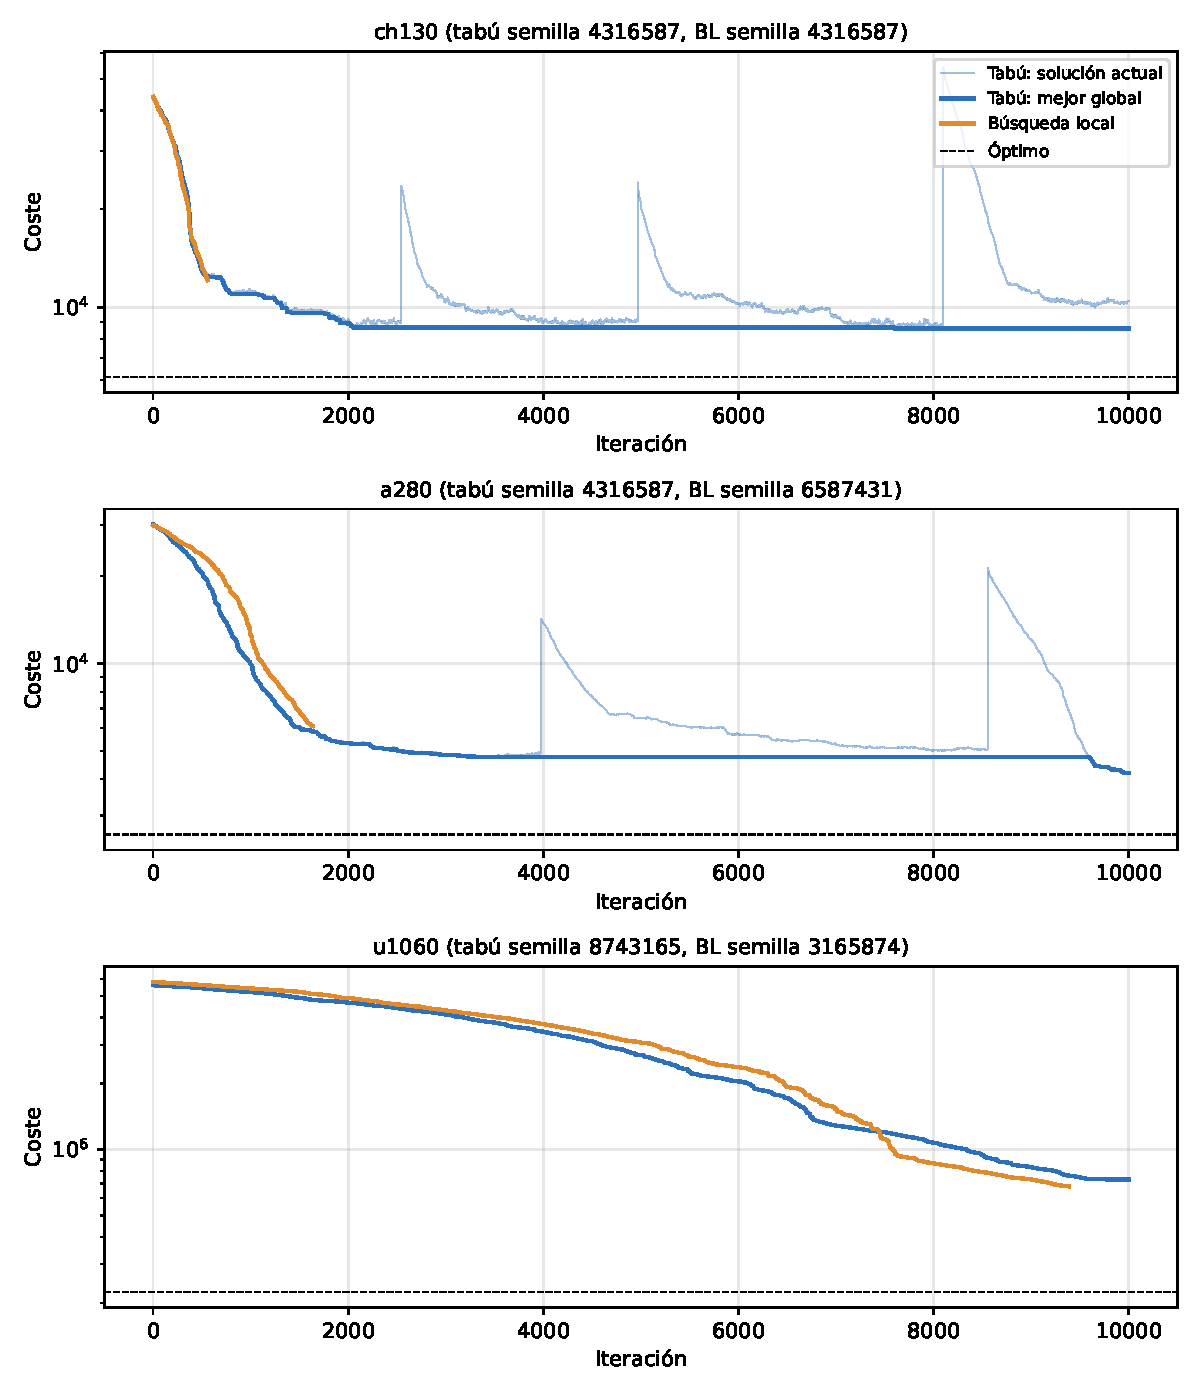
\includegraphics[width=0.92\textwidth]{convergencia.pdf}
\caption{Convergencia de la mejor ejecución de la búsqueda tabú y de la ejecución de la búsqueda local con la misma semilla en ch130, a280 y u1060 (coste en escala logarítmica). La línea fina es la solución actual del tabú y la discontinua, el óptimo.}
\label{fig:convergencia}
\end{figure}

En u1060 el comportamiento es distinto. La búsqueda local necesita entre 9.595 y 9.866 movimientos para llegar a un óptimo local, y en la tercera ejecución se corta en el máximo de 10.000 sin llegar a él. Con el mismo presupuesto, el tabú pasa casi todas sus iteraciones bajando igual que la búsqueda local (entre 0 y 175 empeoramientos y ningún reinicio), por lo que sus mecanismos casi no llegan a actuar. En media queda algo por delante (256,8\,\% frente a 266,8\,\%), aunque la ventaja no es sistemática. Con la misma semilla, el tabú consigue un recorrido mejor en dos ejecuciones (852.455 frente a 881.699, y 730.441 frente a 804.383) y uno peor en la otra (815.905 frente a 780.085). Como la MCP prohíbe algunos movimientos de mejora durante 10 iteraciones y no hay criterio de aspiración, el tabú baja desde el principio por un camino distinto al de la búsqueda local.

En d18512 pasa lo mismo, pero más exagerado, ya que 10.000 iteraciones son muy pocas para 18.512 ciudades. Todas las iteraciones del tabú son de mejora (no hay empeoramientos ni reinicios), y la búsqueda tabú (7.758,9\,\% de desviación media) y la búsqueda local (7.759,1\,\%) acaban prácticamente en el mismo punto, solo un poco por debajo del greedy aleatorio del que parten.

\subsection{Tiempos, desviaciones e influencia del tamaño}

\begin{figure}[H]
\centering
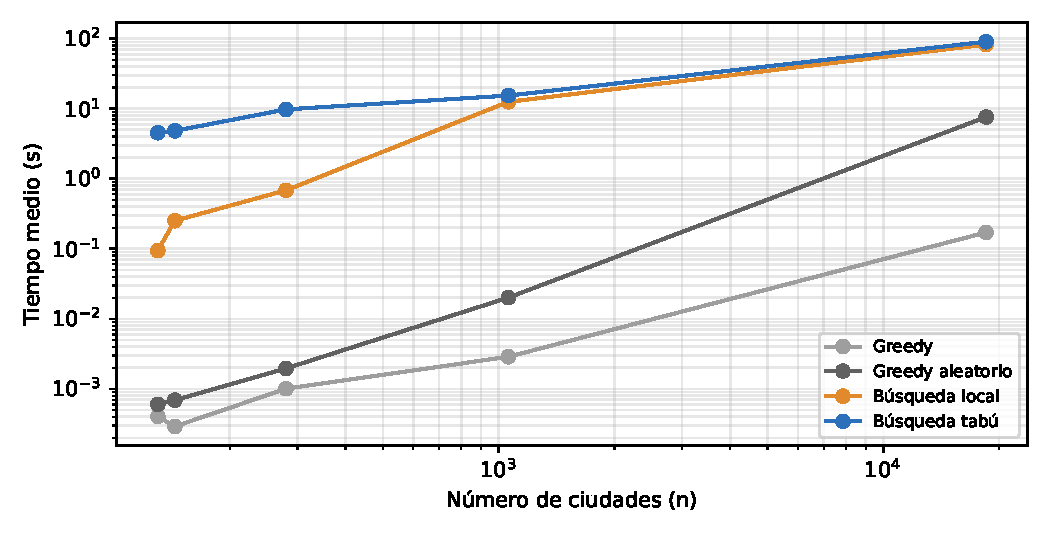
\includegraphics[width=0.8\textwidth]{tiempos.pdf}
\caption{Tiempo medio por ejecución frente al número de ciudades (escalas logarítmicas).}
\label{fig:tiempos}
\end{figure}

El tamaño de la instancia se nota en varios aspectos.
\begin{itemize}
    \item \textbf{Coste de los greedy.} Calcular las sumas de distancias es $O(n^2)$, pero como lo hacemos con operaciones vectorizadas de NumPy el greedy tarda 0,17\,s incluso en d18512. El greedy aleatorio necesita 7,6\,s en esa instancia porque vuelve a ordenar el vector de candidatos cada vez que inserta una ciudad. Solo la matriz de distancias de d18512 ya ocupa alrededor de 1,3\,GB.
    \item \textbf{Presupuesto de iteraciones.} Los movimientos que hacen falta para llegar a un óptimo local aumentan con $n$ (unos 540 en ch130, 1.560 en a280 y más de 9.500 en u1060). Con un límite fijo de 10.000 iteraciones, en u1060 la búsqueda local llega muy justa y en d18512 se queda muy lejos. Las tres ejecuciones de la búsqueda local y las tres del tabú se cortan en 10.000 movimientos con una desviación superior al 7.600\,\%, casi igual que la del greedy aleatorio del que parten. A partir de cierto tamaño, la calidad viene limitada más por el número de iteraciones permitido que por el algoritmo.
    \item \textbf{Tiempo por iteración.} La evaluación factorizada es $O(1)$, pero en cada iteración también hay operaciones $O(n)$, como recalcular el coste o actualizar la MLP, y una exploración del DLB que puede llegar a recorrer $n$ vecinos por posición. Por eso el tabú, que siempre hace las 10.000 iteraciones, tarda en las instancias pequeñas entre 14 y 48 veces más que la búsqueda local, que termina antes. En u1060, donde las dos hacen casi todas las iteraciones, la diferencia baja a 1,2 veces (15,4\,s frente a 12,5\,s). En d18512 ambas agotan las 10.000 y tardan casi lo mismo (90,3\,s frente a 82,3\,s).
\end{itemize}

Con todo esto, en las instancias de hasta unos cientos de ciudades la búsqueda tabú es la que tiene mejor relación calidad/tiempo, porque por unos pocos segundos más que la búsqueda local divide su desviación entre 1,9 y 3,1. En las instancias grandes, con 10.000 iteraciones, ninguna de las búsquedas por trayectorias llega a aprovechar sus mecanismos y las diferencias entre ellas dependen sobre todo de la semilla. No hemos aplicado ningún test estadístico porque con solo tres ejecuciones por algoritmo no tendría potencia suficiente. Aun así, en las tres instancias pequeñas las diferencias entre la búsqueda local y la tabú son mucho mayores que la dispersión entre ejecuciones (Figura~\ref{fig:boxplot}).

\subsection{Análisis de la mejor solución}

Si nos fijamos en la desviación, la mejor solución de todo el estudio es la de la búsqueda tabú en ch130, un recorrido de longitud 7.791,07 que es un 27,5\,\% más largo que el óptimo (6.110). En la Figura~\ref{fig:recorridos} la comparamos con la mejor solución de la búsqueda local en la misma instancia (12.097,10; 98,0\,\%).

\begin{figure}[H]
\centering
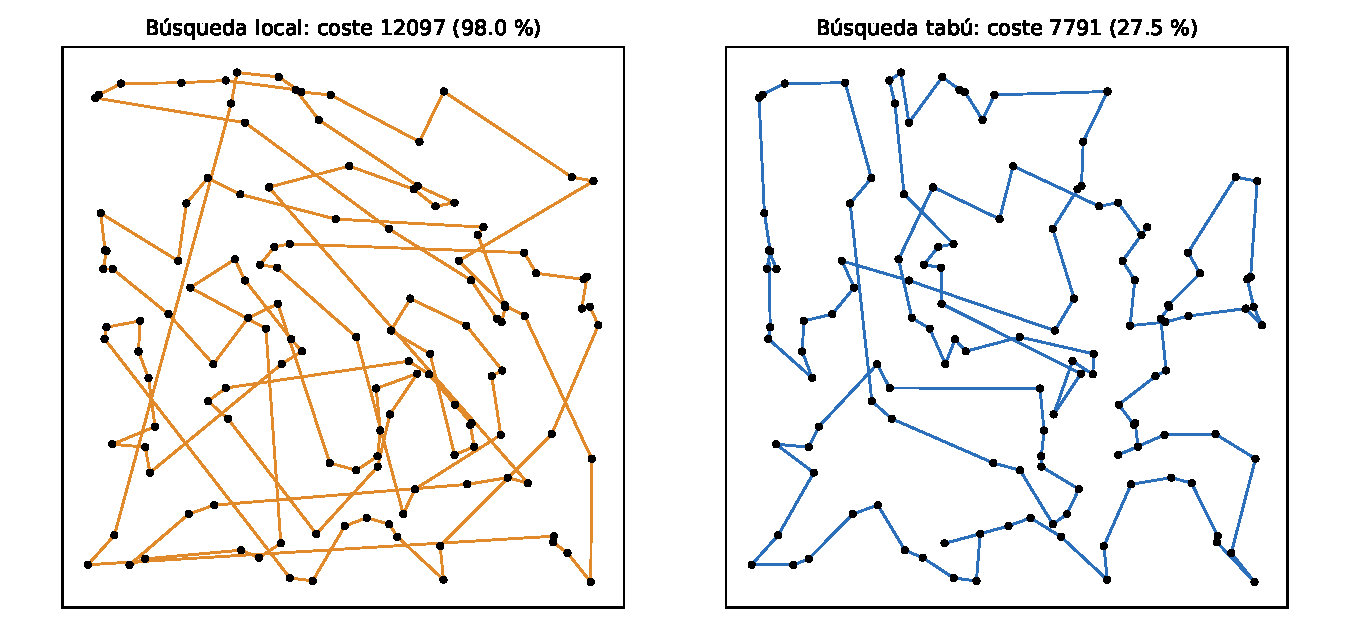
\includegraphics[width=\textwidth]{recorridos_ch130.pdf}
\caption{Mejor recorrido de la búsqueda local y de la búsqueda tabú en ch130.}
\label{fig:recorridos}
\end{figure}

En el recorrido de la búsqueda local hay muchas aristas largas que atraviesan el plano y se cruzan entre ellas. Es un óptimo local para el intercambio de dos ciudades, porque para quitar cada cruce habría que invertir un tramo entero del recorrido y eso no se consigue con un solo intercambio que mejore el coste. El recorrido del tabú, por el contrario, casi siempre pasa de una ciudad a otra cercana y va cubriendo el plano por zonas, aunque todavía le quedan algunos cruces y saltos largos. De ahí viene el 27,5\,\% que falta, ya que con el operador de intercambio no se llegan a eliminar todos los cruces en 10.000 iteraciones ni siquiera aceptando empeoramientos. Una posible mejora sería una variante del operador que, en vez de intercambiar las dos ciudades, invirtiera el tramo del recorrido que hay entre ellas. Con ella se eliminaría un cruce en un solo movimiento y se reduciría esta distancia.

\subsection{Ficheros de registro}

Cada ejecución genera un fichero de log en el que se guardan los parámetros y la semilla, la solución inicial y cada movimiento aplicado con el coste anterior y el nuevo. En la búsqueda local solo hay movimientos de mejora, y en el tabú también de empeoramiento, junto con el mejor del momento actual, el mejor global y el contador de estancamiento. También se registran los reinicios por intensificación o diversificación con su nueva solución y, al final, la solución y el coste finales. Los logs están en la carpeta que se indica en el Anexo.

\section{Referencias}

\begin{itemize}
    \item Material de la asignatura Metaheurísticas, Universidad de Jaén, curso 2026/2027.
    \item Reinelt, G. (1991). TSPLIB --- A Traveling Salesman Problem Library. \textit{ORSA Journal on Computing}, 3(4), 376--384. Óptimos de las instancias: \url{http://comopt.ifi.uni-heidelberg.de/software/TSPLIB95/}.
    \item Glover, F. y Laguna, M. (1997). \textit{Tabu Search}. Kluwer Academic Publishers.
\end{itemize}


\clearpage

\begin{appendices}
  \appendixpage           % página con el título "Anexo"
  \addappheadtotoc        % añade esa página al TOC

  \section{Carpeta de Logs}
Enlace de descarga a la carpeta con los Logs: \url{https://drive.google.com/drive/folders/1JOPyPUdfYNtIpM7BfSW0vkRCTi284ucn?usp=sharing}

Dentro de la carpeta hay un subdirectorio por algoritmo (\texttt{gre}, \texttt{grea}, \texttt{b\_local} y \texttt{tabu}). Los ficheros se llaman \texttt{<instancia>\_<algoritmo>\_<semilla>\_ejecucion\_<n>.log} y en ellos se registran los parámetros, la solución inicial, cada movimiento con su coste (de mejora o, en el tabú, también de empeoramiento), los reinicios por estancamiento, la solución final y un resumen con el coste y el tiempo de la ejecución.

\end{appendices}

\end{document}
